%************************************************
\chapter{Introduction}
\label{chapter:introduction}
%************************************************

In this dissertation I present the substrate for accountable layered
systems.  I have focused on building this substrate for doing
reflective thinking on a large scale in learning systems, using
{\mbox{\citeauthor{singh:2005b}'s~\citeyearpar{singh:2005b}}} example
of reflective architectures as the precedent.  My approach focuses on
a purely procedural approach that does not assume any logical search
algorithms that work behind-the-scenes without a reflective learning
focus.  Without increasing the computational time complexity of basic
search, this approach learns to search in $n$ concurrent layers of
goal-oriented optimization, learning to plan physical actions, while
concurrently learning to plan planning actions, etc.  Physical
activities are presented as analogous to thinking activities, allowing
a recursive application of the model to itself.  The contributions of
this thesis are:

\begin{itemize}
\item \emph{The Model}: A philosophical basis for avoiding tautologies
  while thinking about a grounded model of reflection.
\item \emph{The Simulation}: A mathematical basis in graph theory for
  representing a simulation of the model.
\item \emph{The Substrate}: A computational implementation of three
  working layers of the simulation in a block building domain.
\end{itemize}
  
\section{The Substrate}

The primary contribution is the substrate.  This is a system for
developing large software applications, which enables parallel and
concurrent process control.  The advantage is the system's ability to
selectively pause these parallel processes when bugs are encountered,
so that they can be easily examined in this paused state.
Additionally, there are intricate thread control operations for these
processes.  When they ``sleep'', they are removed from the scheduler,
allowing the substrate to focus computational resources on other
processes.  When required, thousands of sleeping processes can
efficiently be ``triggered'' awake.  The primary point of the system
is that while running many different problem solvers at the same time,
it has the ability to conveniently trace the interactions between
those problem solvers.  Thus, all of the memory in this substrate
allows for the tracing of all memory allocations and mutations.  It is
a frame-based system.  Many AI systems are implemented in an
object-oriented or frame-based representation.  This allows for all of
the commonly associated programming methodologies to exist, i.e.
object types and inheritance, etc.  The substrate includes a
high-level lisp-like programming language, so the compiler can be
redefined by the running program.  There are layered ``cognitive
architecture'' structural primitives included in the language.  This
allows the programmer to build a ``layer'' which contains ``agencies''
which contain ``resources''.  These resources then are able to exist
as ``minds'' which control ``physical worlds'' because these
primitives already exist in this substrate.  This substrate, which can
be downloaded as open-source software, serves as an extensible
platform for continuing research on this implementation of reflective
thinking.

\section{The Simulation}

The second thesis contribution is an example of a mathematical
simulation model that gives answers for the following questions:
\begin{itemize}
\item How do we assign credit to the planning process and learn to
  plan?
\item When many individual processes interact in the solution of a
  common problem, for example, controlling a complicated parallel
  system, how is credit traced for decisions that have been made in
  performing actions?
\item How do we learn what particular knowledge is either good or bad
  at solving different types of problems?
\item How do we trace dependencies back to the point that models of
  planning can be learned?
\item How do algorithms currently assign credit backwards in time and
  how does this model relate to these methods?
\end{itemize}

In this thesis, I evaluate how well this model is able to learn, not
only at the ground level but also at the hypothesis manipulation
level, improving the ground learning performance.  This simulation
will be described as a potential path around the exponential search
explosion problem.  There is a certain ``curse of dimensionality,''
which limits a search algorithm from considering an exponentially
vanishing percentage of the possible search paths as the length of the
paths is increased.  The simulations are often defined in abstract
terms, such as logical relationships, in order to make abstract
simulations of large domains.  Large systems that have logical
relationships require search algorithms to evaluate the implications
of the declarative forms.  These systems fail because there is this
explosion of exponential search.  In my model, in analyzing the
simulation, the curse of dimensionality is reduced through layers of
planned heuristic learning.  My main point is that anything that
involves search can be improved by being in terms of a simulation of
reflective learning.  The details of the simulation model are the
basis of the computational substrate that allows for this improvement.

\section{The Model}

The third thesis contribution is a reflective model of mind that gives
a description of how to think about thinking reflectively.  There are
many models for reflective thinking, and I will compare my model to
other related layered, reflective, and metacognitive models of mind.
The model I describe here has not been explored by many of the current
machine learning disciplines.  Thus, this model will be the basis of
my mathematical simulation.

\section{Document Overview}

{\mbox{\autoref{part:the_model}}} begins with a non-technical
description of the model of mind that is used as the basis of both the
mathematical simulation and the computational implementations.  In
{\mbox{\autoref{part:the_simulation}}}, I explain the modelling
assumptions that I make in transitioning to the mathematical notation
of the simulation model.  Using this notation, I explain how this
model can be used to reduce the complexity of search algorithms.  In
{\mbox{\autoref{part:the_implementation}}}, I give an explanation of
how this simulation is automated on a concurrent computer, the thesis
implementation, SALS, the substrate for accountable layered systems.
In conclusion, in {\mbox{\autoref{part:conclusion}}}, I discuss
promising directions for future research in not only AI but also the
other cognitive sciences.

The focus of the dissertation will be a description of the reflective
problem of learning-to-control.  I describe control in terms of layers
of reflective credit assignment because this simplifies understanding
the problem of learning-to-control.  The focus will be on the
implementation of credit assignment at the level of planning
activities and then describe an example of a computational simulations
of reflective learning in a block building physical domain.

\section{Programming}

An example problem domain called the block building domain is shown in
{\mbox{\autoref{figure:example_problem_domain}}}.  In this case, we
have two blocks, which have relationships with the objects in the
room, such as the table.  If the goal state is to get the physical
world to exist in a particular configuration, the stack of {\tt
  Block-2} on top of {\tt Block-1},
{\mbox{\autoref{figure:example_program}}} shows an example of a
program that a programmer might write to move this gripper around in
this block building domain.  In this program, the gripper has very
simple symbolic commands: {\tt move-right}, {\tt reach}, {\tt grab},
{\tt move-left}, {\tt drop}.  One can imagine that this program might
intend to pick up the green block and put it on the blue block.
\begin{figure}
\center
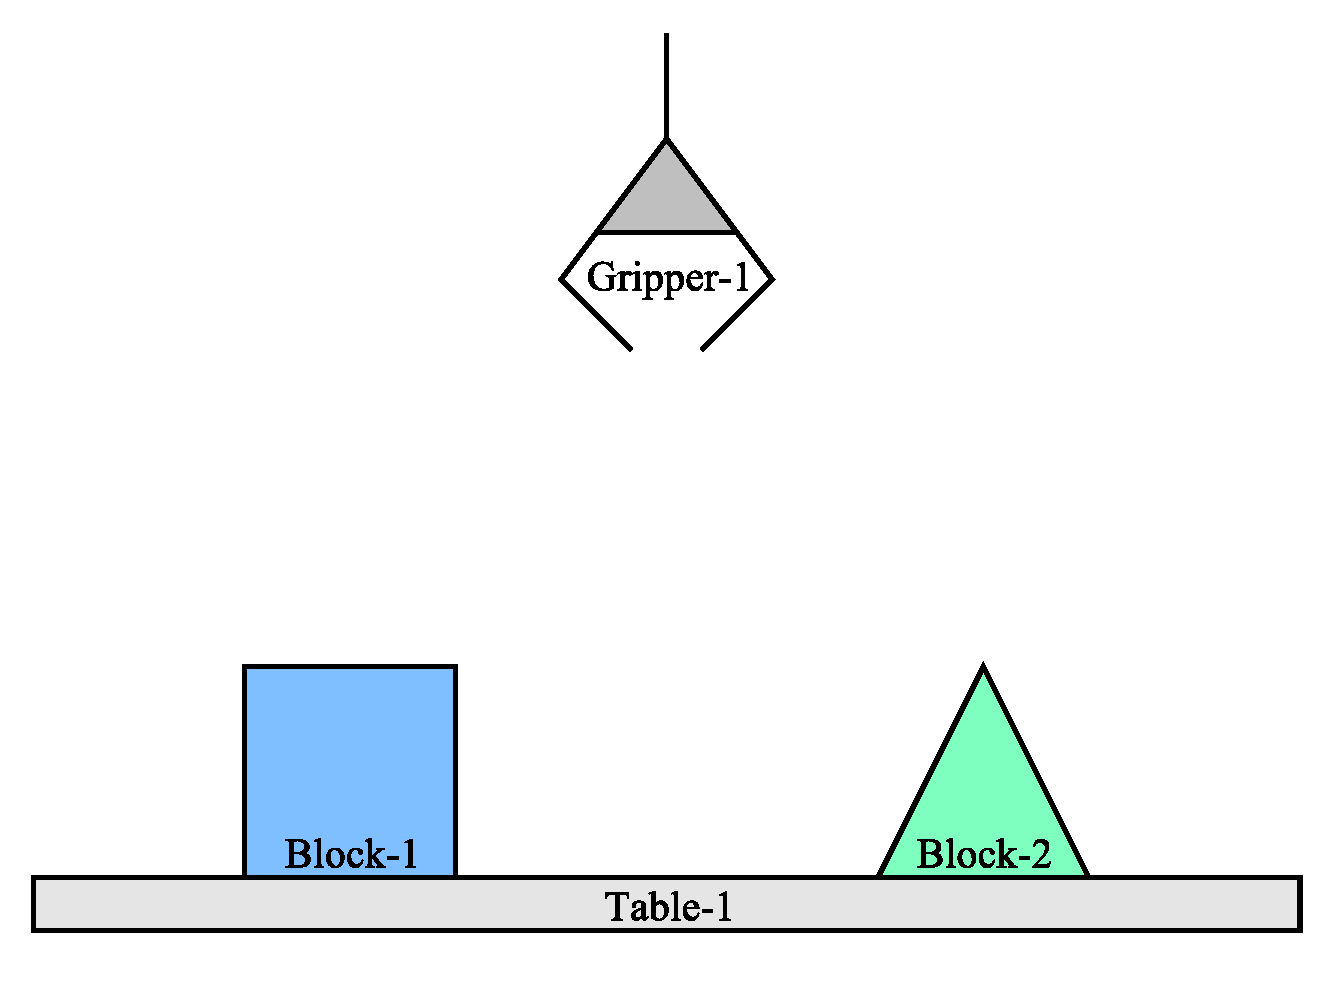
\includegraphics[width=10cm]{gfx/blocks_world_example-1}
\caption{An example problem domain.}
\label{figure:example_problem_domain}
\end{figure}
\begin{figure}
\center
\begin{tabular}{l}
\\
  {\tt ~~[defunk example-program []}~~ \\
  {\tt ~~~~[move-right]} ~~\\
  {\tt ~~~~[reach]} ~~\\
  {\tt ~~~~[grab]} ~~\\
  {\tt ~~~~[move-left]} ~~\\
  {\tt ~~~~[drop]]} ~~\\
\\
\end{tabular}
\caption{An example program.}
\label{figure:example_program}
\end{figure}

\section{State Space Planning}

State space planning can be thought of as automatic programming.
Planning refers to the computer's ability to write its own program.
In an algorithm that plans by using a search algorithm, there is an
initial state with a number of possible actions that may lead away
from this state.  We can move left; we can stop; we can move right.
We can imagine what the possible future states would be after each
action.  In an imagined future state, the gripper may be in a
different position.  An example of the exponential growth resulting
from continuing a planning search is shown in
{\mbox{\autoref{figure:combinatorial_explosion_example}}}.
\begin{figure}
\center
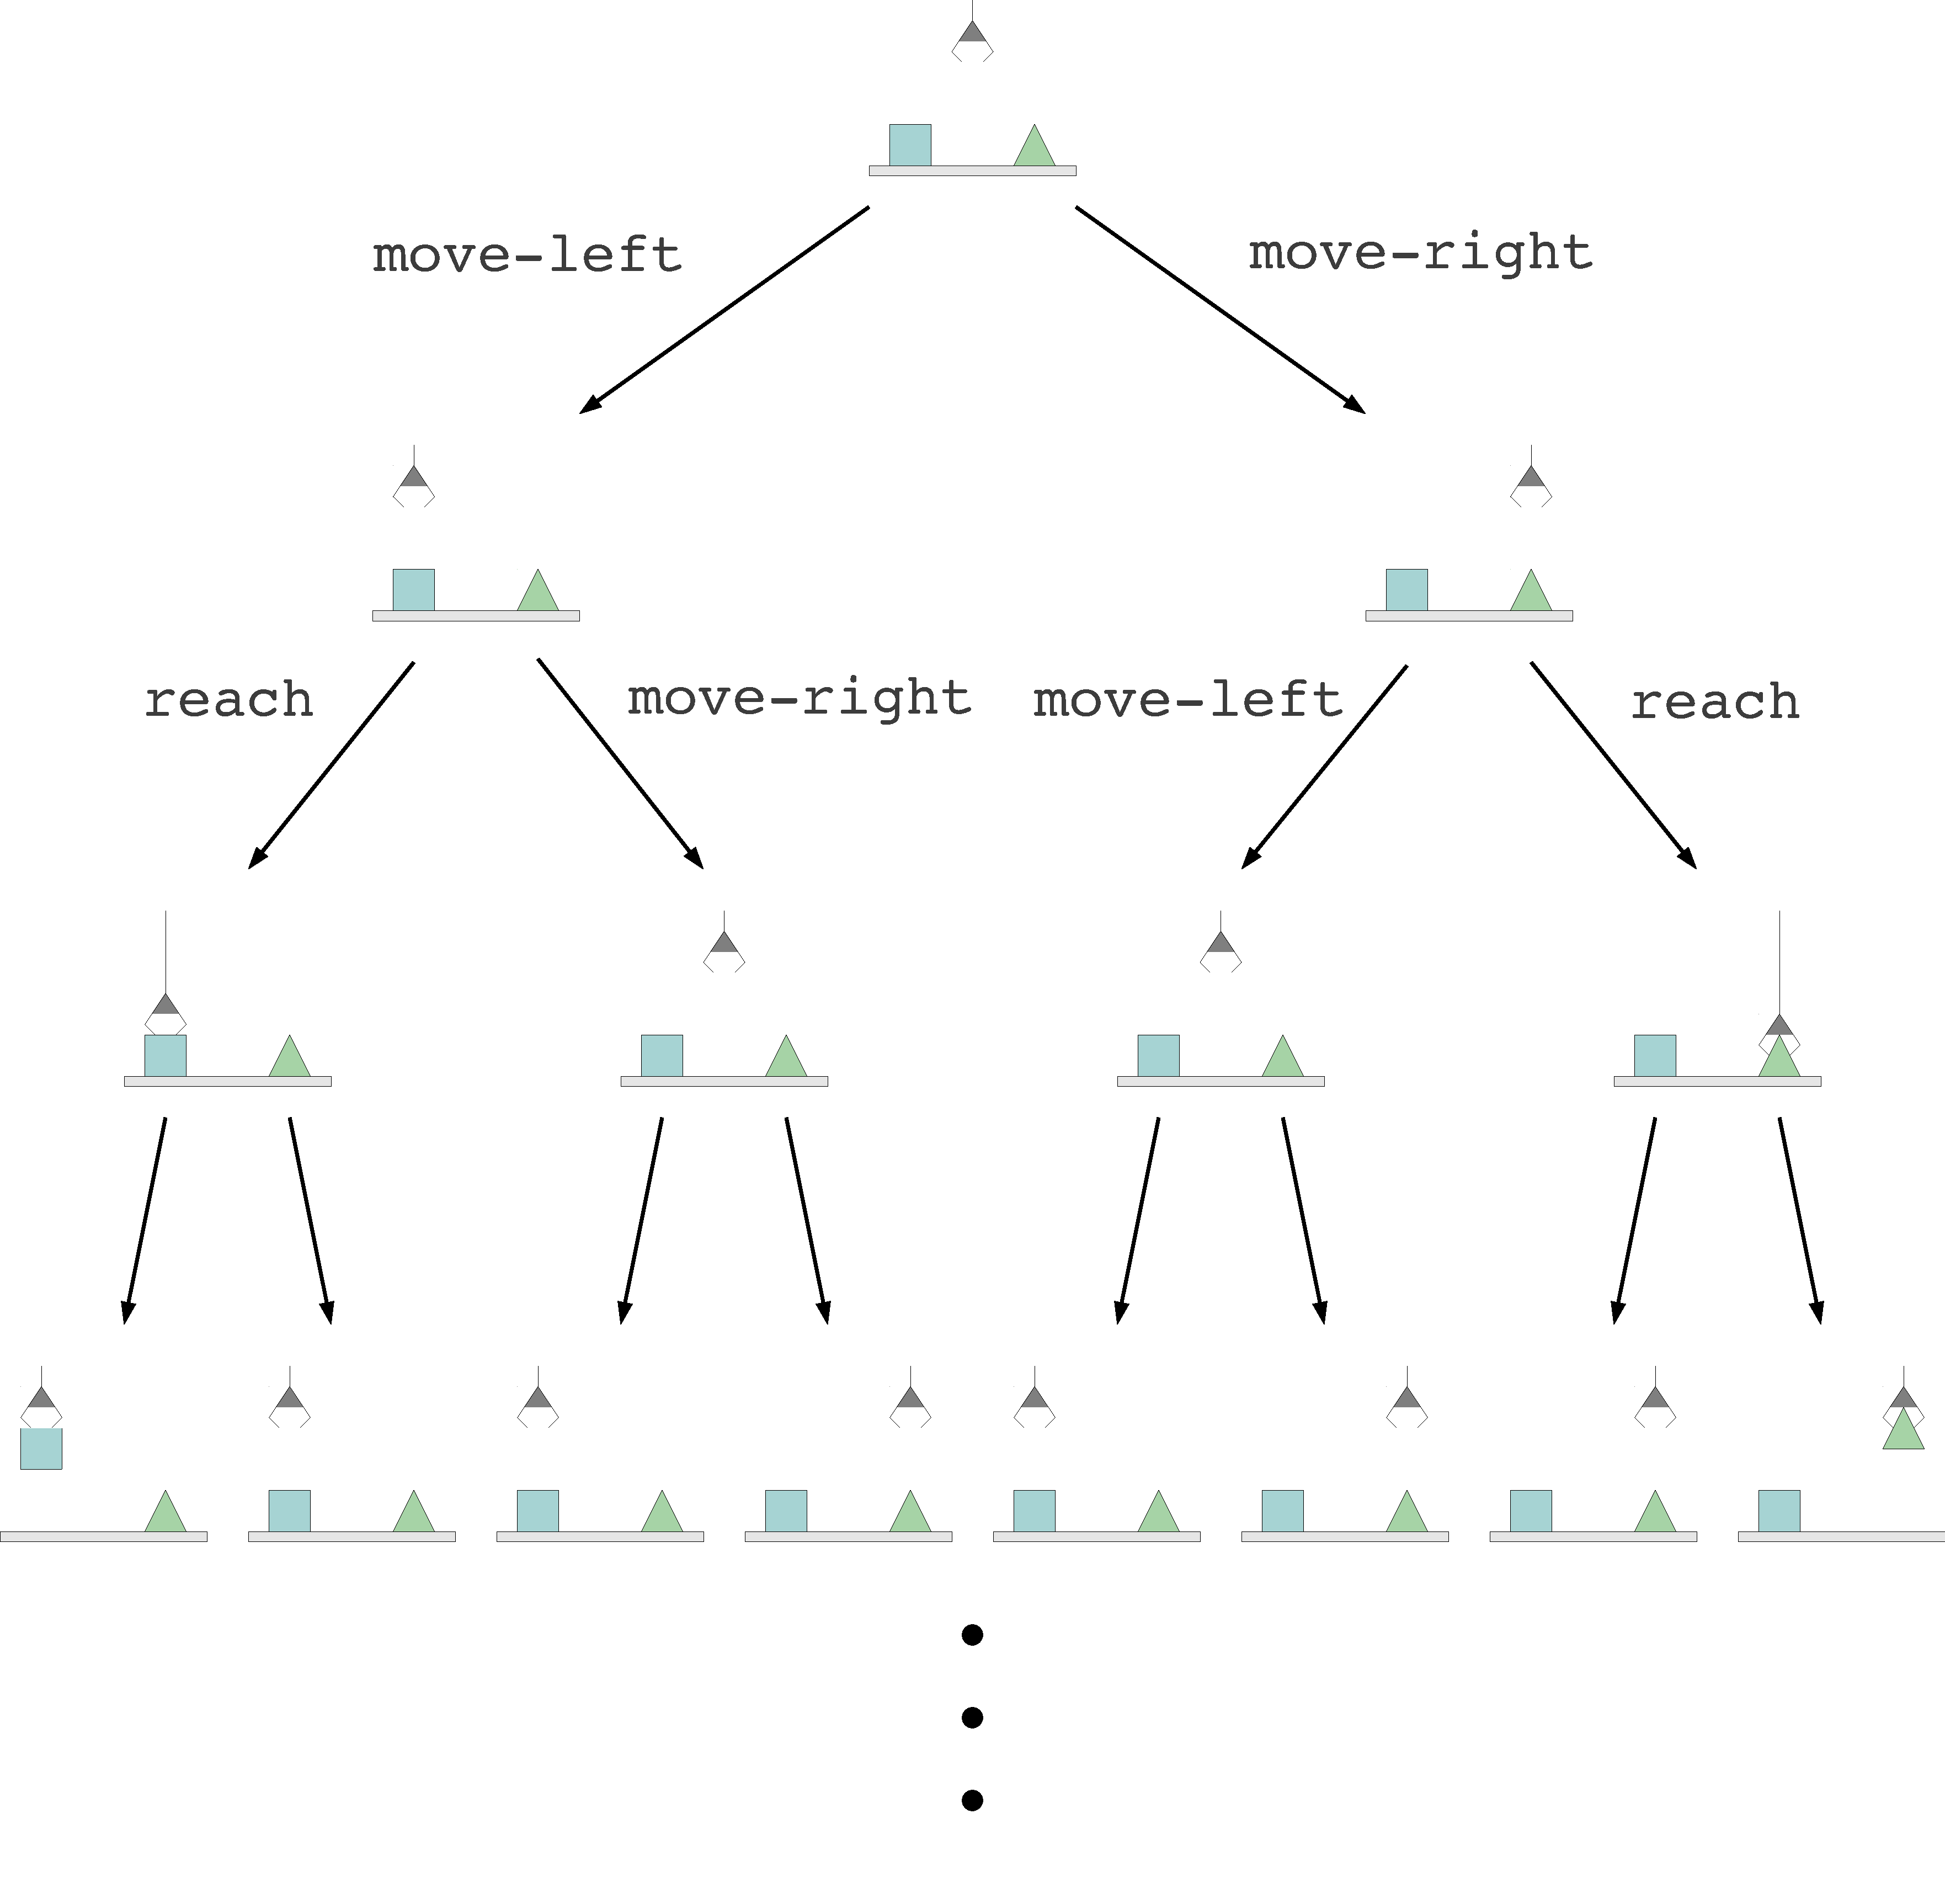
\includegraphics[width=10cm]{gfx/combinatorial_explosion_example}
\caption{Exponential growth in planning as search.}
\label{figure:combinatorial_explosion_example}
\end{figure}
If every considered state in a search has the same number of possible
actions, this search becomes an exponential search problem.  The
number of actions from each state is the \emph{branch factor} of the
search.  Exponential searches quickly become intractable, even in
state spaces with a reasonable number of actions.  For example, games
of chess are played to 20 levels deep with about 30 moves from each
state.  Thus, expanding this search tree gives $30^{20}$, or $3 \times
10^{29}$ plans.  If there were one billion computers that each
processed one billion plans per second in parallel, this search would
still take over ten thousand years to complete, and that is just to
play the first move!  The fastest algorithms include good heuristics,
e.g. a count of the number of pieces on the board for each player,
etc.

\section{Heuristics}

When a problem is exponential, it progresses for as long as can be
afforded computationally, traversing the state space, hopefully
finding the goal state in this large space of all possible
alternatives, but then stops, usually not able to find the required
answer to the problem in the given time or space limitations.
\emph{Heuristics} are one way to alleviate the problematic exponential
growth of the search tree.  In order to search more efficiently,
heuristics provide weightings over the search tree that give a metric
of distance to a completed plan.  Beam search is an example of a
heuristically weighted search that has a finite number of plans that
it considers, forgetting the rest.  As used in beam search, a
heuristic is a function that defines an ordering on search paths.  A
heuristic function defines whether or not a given plan will
successfully accomplish the goal, also, a heuristic gives a metric of
the planning time required until a plan is created that will
accomplish the goal.  The algorithm uses this information to guide the
search, thus reducing the branch factor of the search tree, reducing
the search problem.
{\mbox{\autoref{figure:combinatorial_explosion_example_with_heuristics}}}
shows the same exponential growth example with heuristic weightings
overlayed with blue arrows.
\begin{figure}
\center
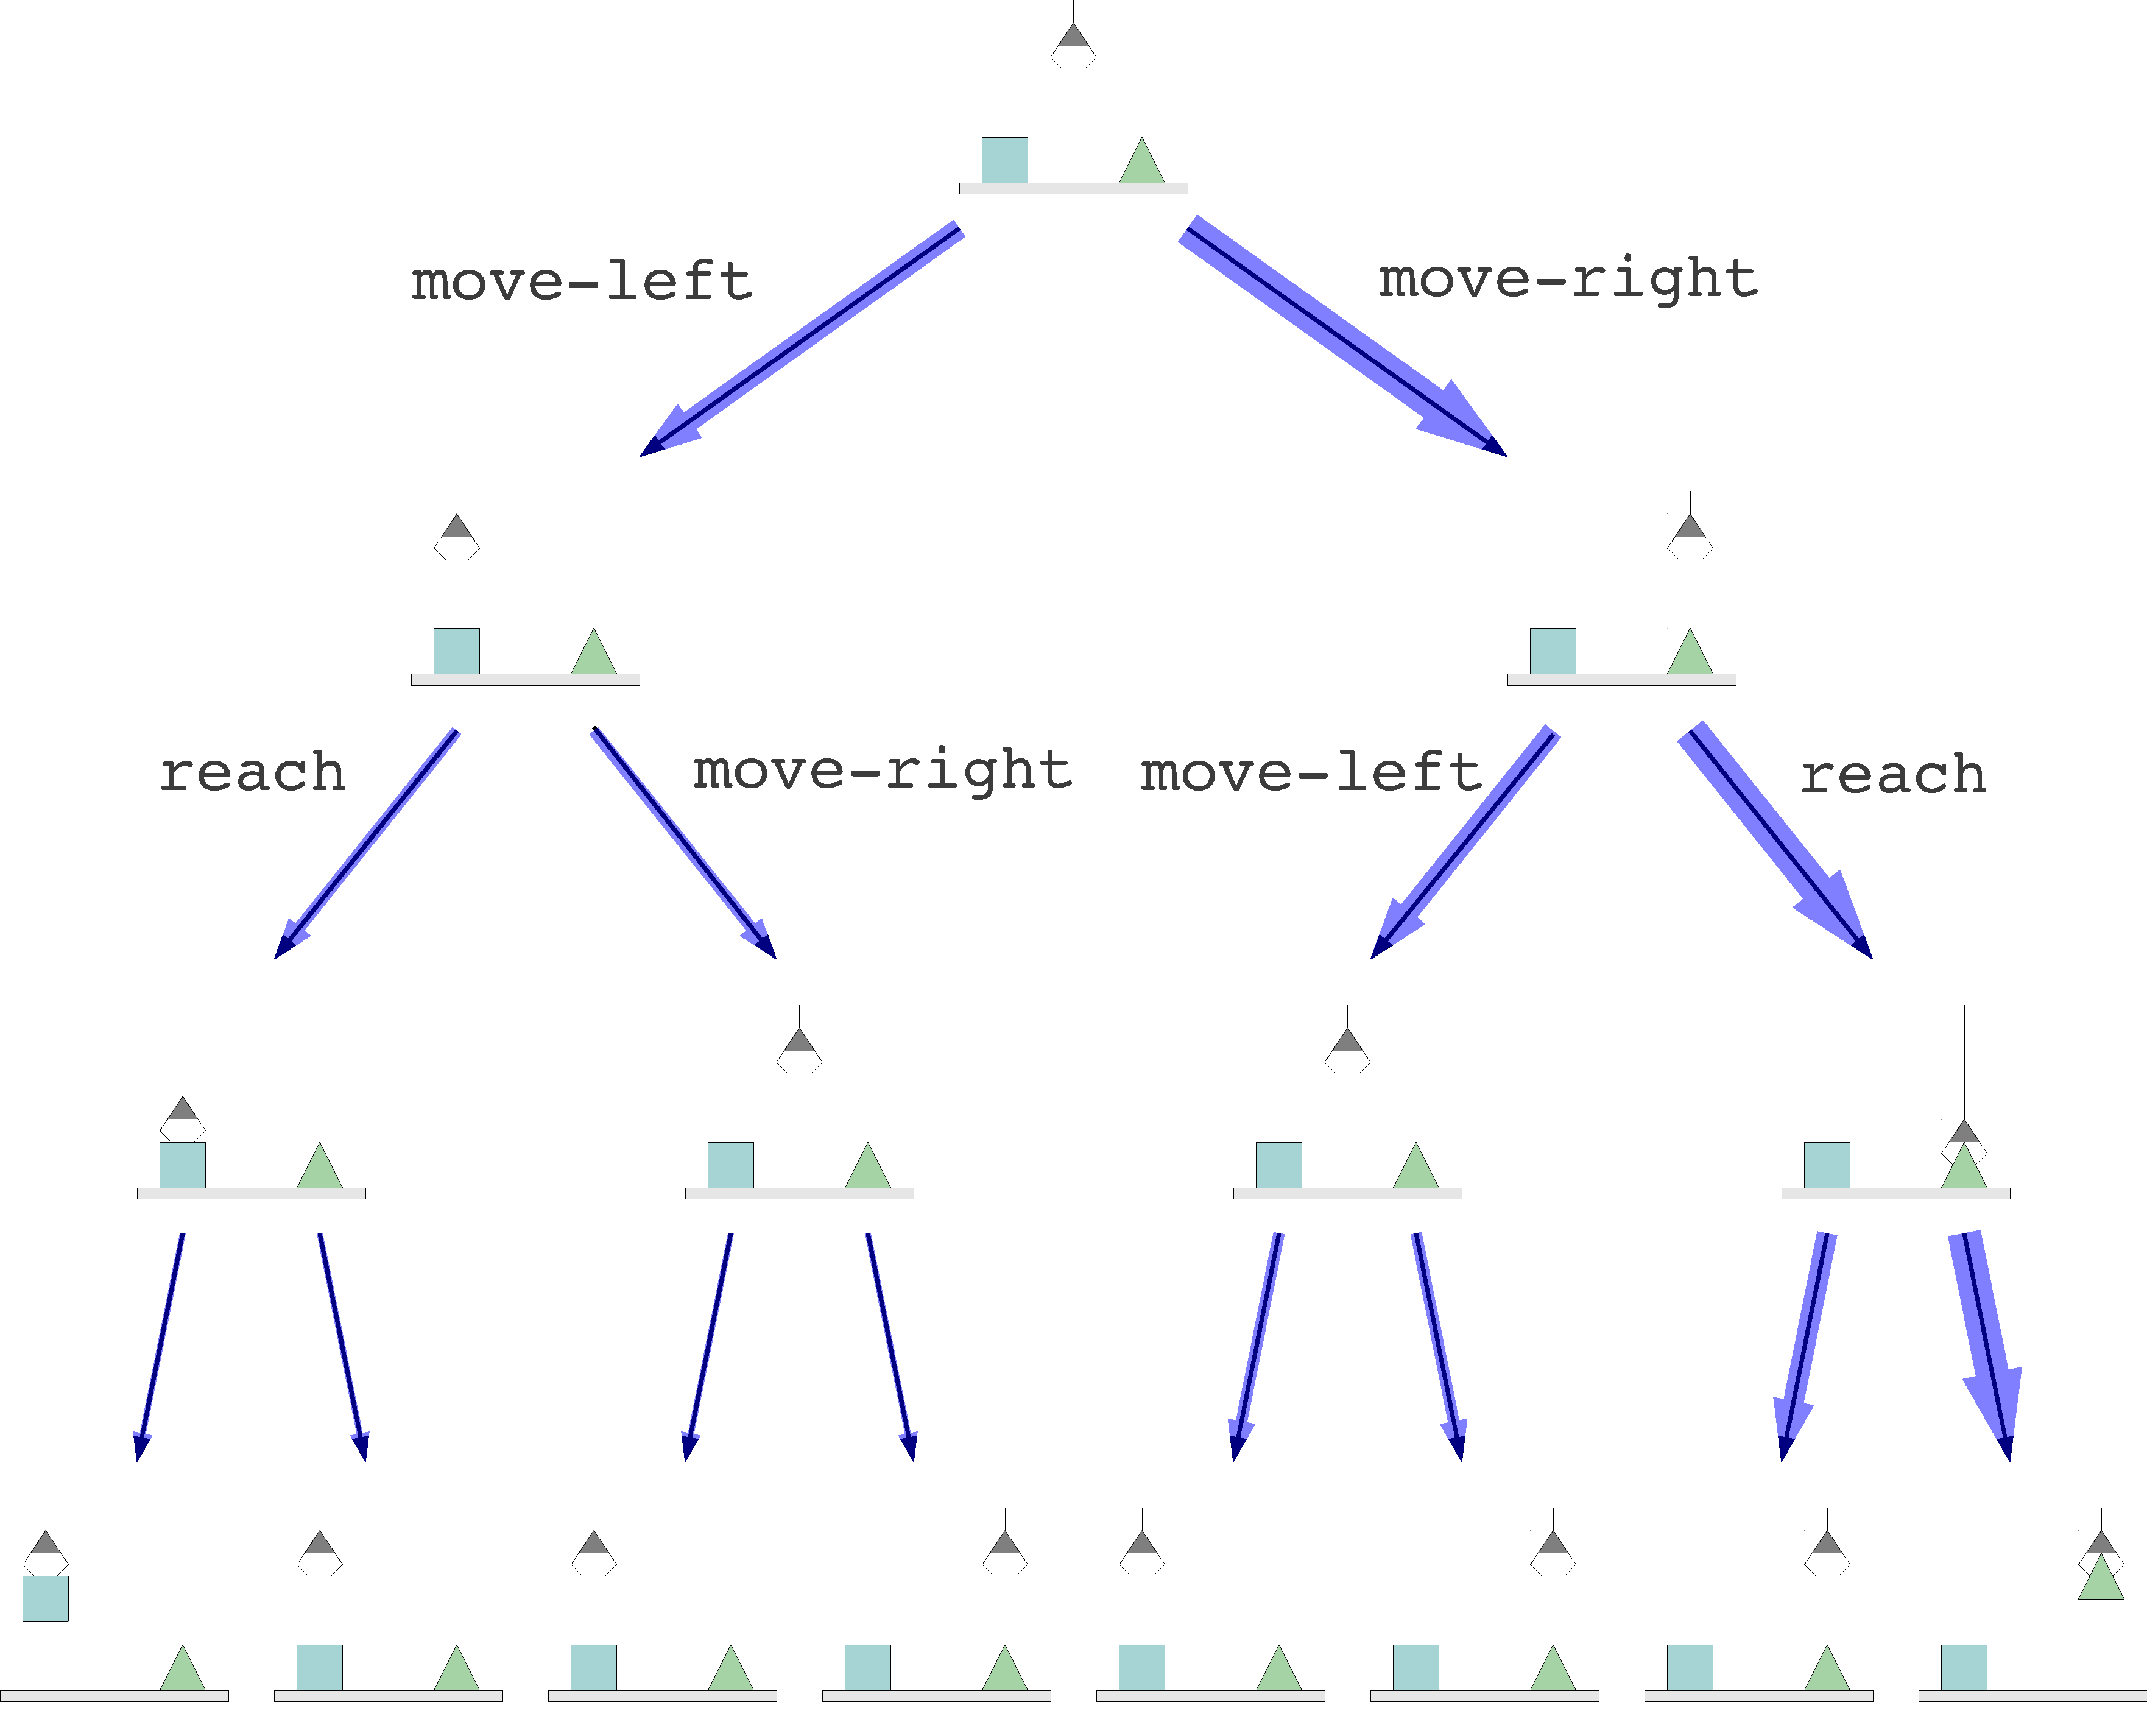
\includegraphics[width=10cm]{gfx/combinatorial_explosion_example_with_heuristics}
\caption{Exponential growth example with heuristics.}
\label{figure:combinatorial_explosion_example_with_heuristics}
\end{figure}

\section{Representing Actions}

The planning as search problem assumes that we have a representation
of the world and a representation for the changes that actions
perform.  Given these models, the physical world can be simulated
according to different plans.  \cite{fikes:1972} describe an action
representation, called ``STRIPS'', that includes an object called a
\emph{transframe} for simulating actions.  In the STRIPS model, the
world is a set of symbols.  A transframe is composed of two sets: one
for the removals from the world and one for the additions to the
world.  A transframe represents a change between two states of the
world.  In a symbolic relational domain, the state space is a set of
symbolic relationships rather than just symbols.  Here is an example
of a symbolic relationship that could exist in a relational domain:
{\tt [block-1 is-on block-2]}.  Here is an example of a transframe for
the world in a relational domain: \emph{remove} {\tt [block-1 on
    table-1]} and \emph{add} {\tt [block-1 on block-2]}.  In
predicting the effects of an action on the world, STRIPS considers one
transframe for each action.  Transframes can also be dependent on the
current state of the world.  Although many function approximation
methods could be used, in my simulation model I have addressed the
problem of learning to predict the correct transframes in the terms of
{\mbox{\citeauthor{mitchell:1997}'s~\citeyearpar{mitchell:1997}}}
``hypothesis spaces,'' which provide a simple and understandable
formulation of the category hypothesis learning problem, given
labelled examples.  Hypothetical models are learned to predict the
effects of actions.  The physical state space informs sets of
hypotheses that can be used to support assumptions, thus, the creation
of new knowledge from an absence of knowledge, given the listed
assumptions.

\section{Learning to Plan for Successful Execution}

Dependency traces for a hypothesized successful plan creation compose
an important set of knowledge to associate with a plan for debugging
the planning process when, later, it is realized that the plan fails
to execute.  {\mbox{\autoref{figure:dependency_traces}}} shows a
picture of dependency traces with hypothesis creation events being
pictured as shapes on a time line.  These hypotheses have arrows
between them that represent the derivation dependencies of each
hypothesis creating decision.  The circles in the picture represent
the symbolic states of the world that are used to create hypotheses,
which are represented by squares.  If any hypothesis is used to derive
another hypothesis, these dependencies give a credit assignment path
that is able to jump back retrospectively an arbitrary distance in
time as well as between reflective layers.  Notice in the picture that
the circle on the far left is a dependency of a square block, but
these two events are not necessarily consecutive in time.  If a
hypothesis is derived from a number of other hypotheses, possibly far
in the past, and this hypothesis fails in action, each one of these
traced dependencies represents a learning opportunity.  Every
additional layer of reflective control in the model, represents
another hypothetical learning opportunity, leading to more efficient
search toward plans that succeed in execution.
\begin{figure}
\center
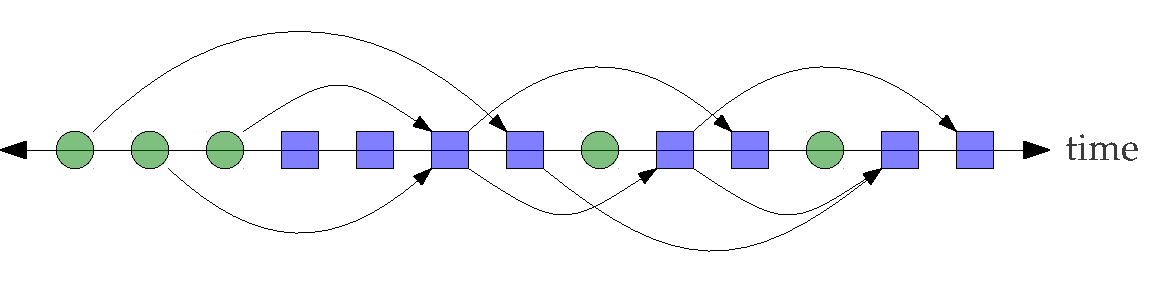
\includegraphics[width=10cm]{gfx/dependency_traces}
\caption[Dependency traces.]{Dependency traces, where circles are
  symbols, squares are hypotheses, and arrows are dependencies.}
\label{figure:dependency_traces}
\end{figure}

\section{Finding a Bug}

The credit assignment problem arises when a bug occurs in some part of
the system.  For example, plans can fail physically to accomplish what
they have been previously hypothesized to accomplish.  There are many
knowledge dependency algorithms that work at this physical knowledge
level.  In this thesis, a layered reflective knowledge representation
is presented for propagating failures to knowledge manipulation
actions as well as physical actions.
{\mbox{\autoref{figure:tracing_bug_dependencies}}} represents a bug
found in a planning hypothesis.  For example, the planning hypothesis
could be that some certain planning activity leads from one type of
plan to a plan that will successfully complete execution without
failing.  Failure propagates through reflective layers of goals and
distinct classes of hypotheses.  Bugs are propagated through every
reflective layer and, therefore, each reflective layer is presented
with a different learning opportunity.
\begin{figure}
\center
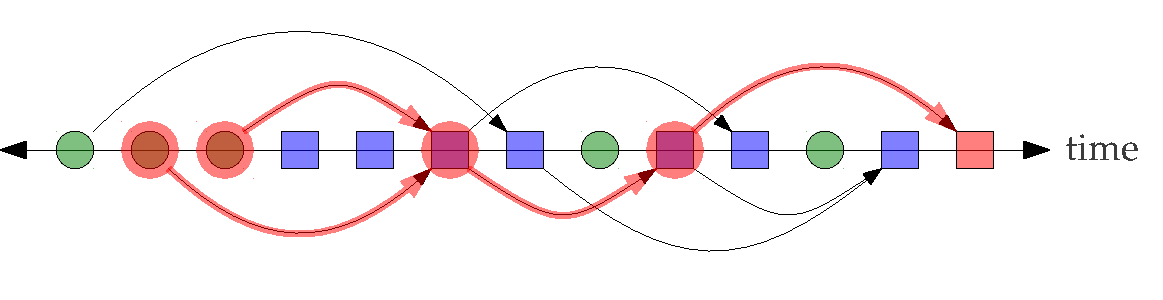
\includegraphics[width=10cm]{gfx/tracing_bug_dependencies}
\caption[Tracing bug dependencies.]{Tracing bug dependencies, where
  the bold arrows represent the credit assignment path for a failure
  in a hypothesis, represented by the red square on the far right.}
\label{figure:tracing_bug_dependencies}
\end{figure}

\section{Comparing Temporal and Reflective Learning}

A reflective learning algorithm implies arbitrarily better learning
algorithms, including one-shot learning algorithms.  In many domains,
the opportunity to learn is rare.  When the cost of failure is high,
it is important to learn as much as possible from each failure.

I will refer to machine learning algorithms that learn by assigning
credit for failures to the temporally previous action as
\emph{temporal learning} algorithms.  Contemporary temporal learning
algorithms are relatively advanced, some even having relational
object-oriented models of actions and the world.  Temporal learning
algorithms learn by assigning credit for a failure to the previous
time step or the previous action.  A reinforcement learning algorithm
that learns in this immediately temporal sense is called the
\emph{temporal difference learning} algorithm as described by
\cite*{kaelbling:1996}.  In temporal learning, the previous action is
considered in the context of the previous physical state of the world.
Preconditions and postconditions for the action are updated.  In other
words, the categories of the world are updated for this action, given
the unexpected reward or punishment, a failure in expectations.  In
the temporal difference learning algorithm, there is a process of
focusing on each previous action and state combination in temporal
order to assign credit for failures.  Temporal learning algorithms
assign credit back, sequentially in time, from action to action.

Reflective learning algorithms can be thought of as having a temporal
learning algorithm within each necessarily distinct layer of
knowledge.  Reflective learning can take advantage of concurrent
processors for each separate layer of activity.  Let $m$ be the number
of reflective layers in a learning algorithm with each layer on a
concurrent processor.  If there is a memory of actions and the state
of the world for the previous $n$ time steps, a temporal learning
algorithm spends $O(n)$ time relearning the effects of the previous
$n$ actions.  The reflective algorithm also spends $O(n)$ time but
relearns the effects of $n*m$ actions, where $m$ is limited by memory
and processors.  Also, if $n$ is $1$, this problem reduces to $1$
learning opportunity for the temporal learning algorithm and $m$
learning opportunities for the reflective learning algorithm.
{\mbox{\autoref{figure:learning_complexities}}} shows a comparison of
the time and space complexities of temporal and reflective learning
algorithms as well as the number of learning opportunities afforded by
one failure.
\begin{figure}
\center
\begin{tabular}{p{2cm}|p{2cm}|p{2cm}|p{3cm}}
Learning Algorithm & Time   & Space      & One-shot Learning Opportunities \\ \hline
Temporal           & $O(n)$ & $O(n)$     & $n$   \\
Reflective         & $O(n)$ & $O(n*m^2)$ & $n*m$ \\
\end{tabular}
\caption{Temporal and reflective learning complexities with one-shot learning opportunities.}
\label{figure:learning_complexities}
\end{figure}

\section{Reflection}

The term reflection is a commonly used word in computer science and
AI.  The idea is extremely simple and is the focus of this thesis,
but, because of its simplicity, it is a widely applicable idea.  In
fact, \cite{maes:1988} distinguishes over 30 different types of
\emph{computational reflection}, grounded in the computer science
literature.  The type of computational reflection that is introduced
in this dissertation is not included in Maes' overview, although the
implementation of this model is based on many of the forms of
computational reflection that Maes does describe, e.g. procedural
reflection, type reflection, frame reflection, and others.  She does
not mention the type of reflection that I am focused on in this thesis
because it was not, at the time, commonly considered computational.
The type of reflection that is modelled here is a psychological type
of reflection: the ability to think about thinking in addition to the
ground problem.  This psychological form of reflection is the focus of
this thesis.

In terms of this model, reflection is the ability to perceive, act,
and plan mental activities.  A planning process is a type of mental
activity, weighing decisions, making plans, and trying to accomplish
goals.  A process that optimizes this planning activity by, for
example, learning heuristics for the planning search, is an example of
a reflective process.  In general, this layered reflective model
learns in reaction to bugs and relearns the planning processes through
dependency tracing for credit assignment.  This model is similar to
current models of \emph{metacognition}, which will be described as
related research.

\section{The Derivative Nature of the Contributions}

The three primary contributions of the thesis are: (1) the
implementation, (2) the simulation, and (3) the model of mind.  My
primary contribution is explained last because it is a derivative of
the first two.  The model of mind is the simplest contribution and
serves as a foundation for the other two.  The simulation model
introduces a discrete state space to the model of mind, so that a
mathematical description can be given of the model of mind.  The
implementation model introduces a computational definition of the
transfer function for the state space introduced in the simulation
model.  Each of these contributions builds on the simpler, prior
contribution.  Therefore, in order to explain the implementation, I
begin with the simplest contribution and work through each additional
component in order to accomplish the primary goal of explaining the
computational implementation of reflective thinking.
{\mbox{\autoref{figure:layers_of_contributions}}} shows the derivative
nature of the contributions of the thesis in the order that they will
be described from most foundational to most abstract.
\begin{figure}
\center
\begin{tabular}{p{3.5cm}p{6.5cm}}
The Model:          & A foundation for how to think about reflective thinking. \\
The Simulation:     & Introduces a discrete state space to the model for a mathematical description of reflective thinking. \\
The Implementation: & Introduces a computational transfer function to the model for automatically simulating the mathematical description of reflective thinking.
\end{tabular}
\caption{The derivative nature of the contributions.}
\label{figure:layers_of_contributions}
\end{figure}

%\section{Hypotheses and Decisions}

%let me just go through a simple example of what a decision is because this becomes very confusing very quickly if we don't ground that idea out.
%this dog looks hungry should i feed him?
%he may bite me.
%this is a basic decision, so let's say we have two options
%how do we think about modelling these two options.
%we're in a current state
%it could possibly lead to two other states
%the question is: what action should we take?
%there is a lot of complicated processing that could into making this decision, but if we just want to talk about the basic development of what a hypothesis is and how do we develop the provenance of data based on that.
%that's what i'm building this up to.
%we have to choose of all of the knowledge we have, maybe from the current state, maybe from the past, which should this decision be based on?
%that's a very complicated problem.
%generally these algorithms are focused on a dataset, so they're not required to learn those types of relationships.
%how should i weigh my relative goals into this decision?
%certain algorithms will have a clear ranking of goals, like a reinforcement learning algorithm will have basically, any time you get into an important state, it will give you an exact number, this state was worth this much.
%this state was worth ten.
%this state was worth negative ten.
%the system that i'm talking about is a little more general than that.
%it uses multiple goals.
%they can have partial orderings.
%but you have to consider, some of the may not even be directly related, so you may have to, part of this decision process could be coming up with that partial order.
%i'd like to dog to not be hungry.
%i also don't want to be bitten.
%you're defining the states of the world that you're going to pay attention to.
%what might be the results of this?
%what might be the relationships?
%what are the relationships now that might help us to make this decision?
%for example, the properties of the dog that we might be paying attention to.
%let's say, there is a hunger for the dog.
%he looks hungry or he looks full.
%these are all things that we're perceiving to make this decision.
%the dog has a color, a breed, it could be barking or not, its going to tell us whether or not the dog is going to bite us basically.
%how do we develop a hypothesis?
%we may have multiple sets of training data.
%this may be our first example.
%we want to take the current situation and we want to make a prediction.
%what kind of hypotheses could we use?
%what does a hypothesis even look like?
%if we feed the dog, there are a bunch of things that might happen.
%he could fall asleep.
%he could continue to be hungry.
%here's a set of examples.
%imagine that we're feeding these examples into the algorithm 1 through 4 on the lefthand side there.
%there are a number of properties that we could then categorize into, for each of these numbered examples we could predict the category on the right.
%we're trying to predict whether or not our hand was bitten given the features on the dog.
%it's basically a function approximation algorithm that we're trying to develop as a hypothesis for this state space.
%
%minsky: mark twain had advice about buying a stock.
%if it goes up sell it.
%if it goes down don't but it.
%
%bo: i think there's a loop in that causal chain.
%i've tried to avoid those.
%
%what's the point?
%why are we talking about this?
%goals!
%because we have goals.
%there are good parts of the world
%there are bad parts of the world
%we want to know how to get to the good parts and avoid the bad parts
%we have avoidances
%we have goals
%we have states of the world
%these might be partial states of the world that we want to pursue or avoid
%deciding on an action depends on weighing these considerations
%what is the state of the world going to be?
%which parts is it going to contain?
%to make this categorization, here's an example.
%very simple algorithm is relatively efficient for doing what it does for getting conjunctions of features as hypotheses for what might predict a category.
%for example, this line here, the first two question marks with "pitbull yes" means "if the statement contains pitbull and it contains that the pitbull is barking then it is categorized as this type of category."
%you can imagine the more general hypothesis is that every dog is going to bite me
%that's all question marks, any of these features match.
%the most specific hypothesis is that none of these features could possibly match
%no matter what feature you tell me its always going to not bite me
%it is a perfectly safe dog.
%these are one example and then two ends of the range of this hypothesis space.
%so, hypothesis h of x is a function that takes state x and predicts whether or not it is an instance of a category.
%what are all of the possible hypotheses that we could learn?
%this is called the inductive bias of the algorithm.
%this is the assumption that we come to the state space with a certain language that we're going to describe our hypothesis within.
%in general this could be a very complicated language.
%in this case its very simple.
%it is just a conjunction of features.
%it helps us to think of these features.
%i'm just going to go over these quickly because this is not fundamental to the theory, but this is just showing that we can efficiently implement a search over the entire hypothesis space.
%we can use a general to specific concept ordering.
%if we consider one concept always predicts that this is a positive category whenever this other concept predicts that its a positive category, then we can say that the hypothesis that predicts it more often is more general than the hypothesis that predicts it less often.
%h 0f j would be the hypothesis that predicts it more often, h of k would be the less often predictor, so there an implication reelationship between every positive instance of h of k to h of j.
%
%making decisions given hypotheses.
%we have collections of these hypotheses that we can efficiently keep track of.
%given training input into this algorithm.
%this is called the version space learning algorithm, which i'm not going into the details of because it isn't important.
%we have hypotheses represented.
%we have collections of every single hypothesis that matches the given training input
%we can efficiently keep track of that
%given a new training instance we can run it through this decision machine to predict what the output is going to be
%when all of our hypotheses agree, we know that we can be confident in our prediction
%when the hypotheses disagree, this is given the assumptions of the version space learning algorithm, which means that the hypothesis that we're looking for is actually in the hypothesis space that we've chosen and things like that.
%if all of the hypotheses agree, then we know that this is the right answer.
%the hypothesis is in that space and it would also agree.
%when the hypotheses disagree it becomes a lot more interesting.
%so, how do we make decisions?
%it could go one of two possible ways depending on if our hypothesis is in one set or the other, but we still act
%we make some kind of assumption there.
%there are probabilistic formulations of this for decision theory that says "all of my hypotheses are equally likely"
%you need a prior on your hypothesis space that gives some kind of weighting on these things so that you can make a decision
%there are 10 hypotheses that say yes there are 5 that say no, given that they're all equally probable, i'm going to take the one that says yes.
%you can make those decisions.
%you can apply those assumptions to this algorithm.
%
%in any case, you do have to make a decision, if you do make the decision which is useful, then you can keep track of that decision's knowledge.
%yes, i'm going to imagine this state of the world.
%you can associate with that knowledge the hypotheses used to generate it.
%you can even imagine going both ways.
%if you consider that both of these are possible outcomes, you can imagine both possible states given the hypotheses that derive them.
%we understand decision making.
%the definition of the hypothesis is relatively clear.
%the tracing the provenance of data is relatively clear.
%
%the causal tracing of processes.
%this is the low level computer science graphic of how you would trace a process.
%we have low level commands or events that we are told to execute.
%this is a normal AI program that is just running without reflection.
%we can imagine a loop being hardcoded into this algorithm, a sequence of events that has pointers back to loop.
%there's the process sitting there in memory.
%we can run this process.
%we can take a virtual machine.
%this is loading the process into the execution register of the machine.
%it starts running.
%that's all the execution register knows how to do.
%it just interprets and starts running.
%this is what a normal AI system will do.
%you load the program into the processor and it executes the program.
%what we've added to this is the creation of semantic events.
%when something important happens in the process below, we create a sequence of semantic events.
%things that might be important to keep track of.
%this function is just beginning its an important function so maybe you should know about that.
%that function has exited successfully.
%there were not bugs in it or i wouldn't have gotten here.
%keeping track of all of these kinds of events can give us knowledge to reflect over the process.
%its a basic low level computer science, computational reflection.
%i'm going to distinguish that from the psychological word of reflection which i'm going to use to refer to controlling the deliberative process.
%we keep track of these semantic events, which then we can recognize.
%oh this pattern looks like this function is entering.
%this function looks like this function is executing.
%we can then have responses that happen in parallel to the basic running process.
%there is an efficiency thing that we can talk about here.
%the tracing of the events require a constant time slowdown.
%algorithmically, that isn't a slowdown, theoretically, its big O notation.
%this algorithm is running the same speed and now we've added computational reflection to it.
%
%gjs: what is this diagram showing?
%i'm confused.
%
%bo: there is a list of.  we can think of these as low level instructions to a machine, like bytecode operations.
%
%gjs: yes.
%
%bo: these bytecodes have a jump from the C to the W there.
%
%gjs: right.
%
%bo: this virtual machine is like a thread.
%
%gjs: yes.
%
%bo: you can load this program in to have the thread start running it.
%then on the top we can keep track of a trace of semantic events.
%
%gjs: i'm confused about these top things that look like a sliding R on a little device I could carry around.
%
%bo: this is meant to be a physical analogy.
%it's kind of like chemistry with the dna.
%
%gjs: i'm trying to figure out what its an analogy to.
%what are you trying to actually
%
%bo: right.  let me describe the analogy and then i'll describe how its implemented.
%the analogy is that we have dna.
%we have transcriptase running along the rna
%and its creating amino acids that end up folding into proteins.
%what this end up doing is it reads along this chain and its creating this string, which is basically, these are the amino acid codons that i want to be attaching to me.
%
%gjs: is the string the one in the purple?
%
%bo: the string is the one in the purple.
%
%gjs: yes, okay.
%
%bo: these are the codons that i want to attach.
%these basically represent the amino acid binding.
%
%gjs: these things on top are patterns.
%is that what they are?
%
%bo: these are patterns.
%
%gjs: they match something?
%
%bo: right.
%
%gjs: ah.  thank you.
%
%bo: they're meant to be floating around and then they float down and bind to the string.
%
%gjs: okay.
%
%bo: this is the physical analogy.
%how that's implemented is you have a stream with multiple listeners each one recognizing a pattern.
%
%gjs: fine.
%
%bo: i use the physical analogy because there's parallel processing.
%you can imagine the basic transcriptase running along the molecule without worrying about slowing down the other molecules around it in their physical simulation.
%we can have responses that are other processes that immediately begin running concurrently.













